% 几何准确：a=1.8,b=1.1; P=(a,0); A=(a,b); B=(a,-b)
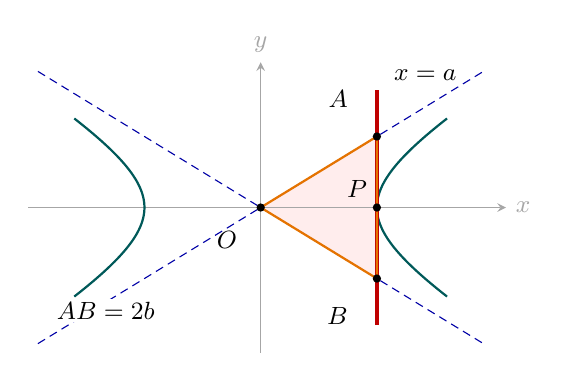
\begin{tikzpicture}[x=0.82cm,y=0.82cm,>=stealth,
  every node/.style={font=\small}]
\def\aa{1.8}\def\bb{1.1}
\coordinate (O) at (0,0); \coordinate (P) at (\aa,0);
\coordinate (A) at (\aa,\bb); \coordinate (B) at (\aa,-\bb);
\fill[red!7] (O)--(A)--(B)--cycle;
\draw[gray!70,->] (-3.6,0)--(3.8,0) node[right] {$x$};
\draw[gray!70,->] (0,-2.25)--(0,2.25) node[above] {$y$};
\draw[densely dashed,blue!65!black] (-3.45,-2.108)--(3.45,2.108);
\draw[densely dashed,blue!65!black] (-3.45,2.108)--(3.45,-2.108);
\draw[teal!70!black,thick,domain=-1.05:1.05,samples=80,variable=\t]
 plot ({1.8/2*(exp(\t)+exp(-\t))},{1.1/2*(exp(\t)-exp(-\t))});
\draw[teal!70!black,thick,domain=-1.05:1.05,samples=80,variable=\t]
 plot ({-1.8/2*(exp(\t)+exp(-\t))},{1.1/2*(exp(\t)-exp(-\t))});
\draw[red!75!black,ultra thick] (\aa,-1.82)--(\aa,1.82);
\draw[orange!90!black,thick] (O)--(A)--(B)--cycle;
\fill (O) circle(1.5pt) node[below left=5pt] {$O$};
\fill (P) circle(1.5pt) node[above left] {$P$};
\fill (A) circle(1.5pt) node[above left=7pt] {$A$};
\fill (B) circle(1.5pt) node[below left=7pt] {$B$};
\node[align=left,fill=white,inner sep=1pt] at (-2.4,-1.6) {$AB=2b$};
\node[align=left,fill=white,inner sep=1pt] at (2.55,2.05) {$x=a$};
\end{tikzpicture}
